% Complemento C1: Transformaciones proyectivas
% Números del pentágono y de la razón doble: apunte/scripts/capc1_proyectivas.py
% Números y figura del conjugado armónico: apunte/scripts/capc1_conjugado_armonico.py
% Números y figuras de la aplicación (la fachada): apunte/scripts/c1_proyectivas.py
\capituloComplemento[1]{Transformaciones proyectivas}\label{cap:proyectivas}\label{sec:bloque-proyectivas}


\section{La idea}

Mirá la sombra de una reja al mediodía, sobre el piso del patio. ¿Los barrotes de la sombra
siguen siendo paralelos? Sí: los rayos del sol llegan prácticamente paralelos entre sí y la
sombra es una afinidad de la reja, como las del capítulo~\ref{cap:afines}.
Ahora prendé de noche una lámpara cerca de la misma reja. ¿Qué les pasa a las sombras de los
barrotes? Se abren en abanico: siguen siendo rectas, pero dejaron de ser paralelas.
Pensá en las vías del tren vistas desde el andén: ¿dónde se juntan dos rieles que en el
terreno nunca se tocan? En un punto del horizonte que se llama \emph{punto de fuga}: en la
imagen, dos paralelas se cortan.
Sacale una foto de costado, y un poco desde abajo, a una pared con una ventana rectangular.
¿La ventana sale rectangular en la foto? ¿Los lados opuestos siguen paralelos?
¿Podés medir sobre la foto, con una regla, el ancho de una puerta de la misma pared?
Mirá qué sobrevivió: las rectas de la pared siguen siendo rectas en la foto, y un punto que
estaba sobre una recta sigue sobre ella.
¿Alcanza con eso para deshacer la perspectiva y ver la pared de frente? ¿Cuántos puntos de la
pared hay que reconocer en la foto para lograrlo?

Esas preguntas arman el complemento. En la cadena de familias del
capítulo~\ref{cap:afines} quitamos ahora la última condición: una transformación
\emph{proyectiva} conserva rectas y nada más. Para qué sirve: describe lo que hace una cámara
con una superficie plana (una pared, un terreno) y permite deshacerlo. Mostramos que cuatro
puntos la determinan, que hay un número que se conserva, la \emph{razón doble}, y la ubicamos
en la jerarquía de transformaciones del plano. Al final enderezamos la foto de la pared y
medimos la puerta (sección~\ref{sec:c1-aplicacion-fachada}).

\subsection{Transformaciones proyectivas: conservar rectas, nada más}\label{sec:proyectivas-primera}

{\small\vspace{1mm}\linkUnidad{05_proyectivas}{Simulación interactiva: Unidad 7 — Proyectivas: la perspectiva de una cámara y el pentágono regular}\par}


Las transformaciones proyectivas mantienen las rectas como rectas y, por eso, quedan
definidas por un cuadrilátero. La imagen mental es la toma de una cámara. Una cámara inclinada sobre un
terreno plano convierte un lote rectangular en un trapecio: los alambrados paralelos
convergen hacia un punto de fuga, las distancias no se conservan en ninguna proporción fija,
y sin embargo toda recta del terreno sigue siendo una recta en la foto. Esa es la única
propiedad que sobrevive, y es la que define a la familia.

\begin{idea}[Qué agrega la perspectiva]
Las afinidades conservan rectas \emph{y paralelismo}. Las transformaciones proyectivas
conservan rectas \emph{solamente}: dos paralelas pueden dejar de serlo y cortarse en un punto
de fuga; un punto ordinario puede irse al infinito y un punto ideal puede volverse ordinario.
Las afinidades son un caso particular de las proyectivas.
\end{idea}

En coordenadas homogéneas la diferencia es mínima y muy visible. Llamamos \(H\) a la matriz
de \(3\times3\) que transforma la terna \((x,y,1)^T\) de un punto y \(X,Y,W\) a las tres
coordenadas de la terna que resulta; \(W\), la tercera, es la que decide la escala. Una
afinidad tiene matriz con última fila \((0,0,1)\), de modo que \(W\) siempre vale \(1\). Una transformación
proyectiva tiene una matriz \(3\times3\) invertible \emph{cualquiera}:
\[
\begin{pmatrix}X\\Y\\W\end{pmatrix}=H\begin{pmatrix}x\\y\\1\end{pmatrix},
\qquad
(x',y')=\left(\frac{X}{W},\frac{Y}{W}\right).
\]
Ahora \(W=h_{31}x+h_{32}y+h_{33}\) depende del punto, y la división por \(W\) es
exactamente la perspectiva: lo que \enquote{está lejos} se achica. Los puntos con \(W=0\) forman
una recta que se va al infinito, el horizonte de la foto.

\paragraph{Por qué un cuadrilátero.}
La matriz tiene nueve entradas, pero \(H\) y \(\mu H\), con \(\mu\neq0\), representan la misma
transformación (el factor se cancela al dividir por \(W\)). Quedan ocho números
independientes. Cada correspondencia \enquote{el punto \(p\) va al punto \(p'\)} aporta dos
ecuaciones, una por coordenada. Cuatro puntos, sin tres alineados, dan ocho ecuaciones: la
transformación queda determinada. Con tres puntos falta decidir \enquote{cuánta perspectiva hay};
un quinto punto ya no se puede prescribir: va a donde la transformación determinada por los
otros cuatro lo mande.

\paragraph{Puntos fijos.}
Un punto es fijo cuando \(Hp=\lambda p\): un autovector de \(H\). El polinomio característico
tiene grado \(3\), y un polinomio real de grado impar siempre tiene una raíz real. Por lo tanto
\textbf{toda transformación proyectiva del plano tiene al menos un punto fijo}, que puede ser
un punto ordinario o un punto ideal (una dirección fija, como en una traslación).

\begin{idea}[Puntos fijos del plano = subespacios invariantes de \(\R^3\)]
En coordenadas homogéneas, una transformación afín o proyectiva del plano es una
transformación lineal de \(\R^3\). Sus subespacios invariantes corresponden a los elementos
fijos en \(\mathbb{P}\R^2\): una recta invariante por el origen de \(\R^3\) es un punto fijo,
y un plano invariante es una recta fija.
\end{idea}

\subsection{Jerarquía de transformaciones del plano}\label{sec:jerarquia}

El cuadro completo de qué conserva cada familia, con sus grados de libertad y los puntos
homólogos que la fijan, está en la sección~\ref{sec:mapa-transformaciones}
(cuadros~\ref{tab:conserva} y~\ref{tab:ficha}): cada familia contiene a la anterior y conserva
menos, y la proyectiva es la última de la cadena. Acá interesa lo que le pasa a ella.

\emph{Por qué se pierde el paralelismo.} Dos rectas paralelas de dirección \(d\) comparten su
punto impropio \((d_1,d_2,0)^T\) (definición~\ref{def:06-impropio}). Una afinidad, con última
fila \((0,0,1)\), lo manda a \((Ad,0)^T\), otro punto impropio: las imágenes siguen paralelas.
Una homografía lo manda a \(H(d_1,d_2,0)^T\), cuya tercera coordenada es
\(h_{31}d_1+h_{32}d_2\), en general distinta de cero. Entonces las dos rectas imagen comparten
un punto \emph{ordinario}, el punto de fuga, y se cortan ahí. Solo la dirección con
\(h_{31}d_1+h_{32}d_2=0\) conserva sus paralelas.

\emph{La recta del infinito.} Los puntos impropios forman una recta, la recta ideal
\(W=0\), de coordenadas \(\ell_\infty=(0,0,1)\). Como las rectas se transforman con
\(H^{-T}\), la homografía la lleva a la recta \(H^{-T}\ell_\infty\), que es ordinaria salvo que
\(h_{31}=h_{32}=0\): en la foto, el horizonte. Al revés, la recta
\(h_{31}x+h_{32}y+h_{33}=0\) del plano va a parar a la recta ideal. Una afinidad deja fija la
recta ideal, y por eso no tiene puntos de fuga.

\emph{La razón doble, único invariante numérico.} Restringida a una recta, una homografía es
\(x\mapsto(\alpha x+\beta)/(\gamma x+\delta)\), y toda función de esa forma con
\(\alpha\delta-\beta\gamma\neq0\) se obtiene así: sobre la recta \(y=0\), la matriz
\(\left(\begin{smallmatrix}\alpha&0&\beta\\0&1&0\\\gamma&0&\delta\end{smallmatrix}\right)\)
lleva \((x,0,1)^T\) a \((\alpha x+\beta,\ 0,\ \gamma x+\delta)^T\). En particular, para tres
puntos distintos \(a,b,c\) de la recta,
\[
  g(x)=\frac{(x-a)(b-c)}{(x-c)(b-a)}
\]
es una homografía que los lleva a \(0\), \(1\) y \(\infty\). Si un número \(I(a,b,c,d)\)
calculado con cuatro puntos alineados no cambia por homografías, entonces
\(I(a,b,c,d)=I\bigl(0,1,\infty,g(d)\bigr)\): depende solo de \(g(d)\), y
\(g(d)=1/\bigl(1-(a,b;c,d)\bigr)\), como se comprueba restando
\(1-(a,b;c,d)=\frac{(a-b)(d-c)}{(c-b)(d-a)}\). Todo invariante numérico de cuatro puntos
alineados es, entonces, una función de la razón doble (proposición~\ref{prop:c1-razon-doble}).
Las distancias, los ángulos, las áreas y las razones simples no lo son, y se pierden.

\section{Construcciones, cuentas y ejemplos}

Escribimos la homografía como una matriz de \(3\times3\), mostramos que cuatro puntos la determinan y buscamos sus puntos y rectas fijas. Cerramos enderezando la foto de una fachada.

{\small\vspace{1mm}\linkUnidad{05_proyectivas}{Simulación interactiva: Unidad 7 — Proyectivas: la perspectiva de una cámara y el pentágono regular}\par}
{\small\vspace{1mm}\linkAnimacion{02_homogeneas_pentagono_3d}{Animación: el pentágono en coordenadas homogéneas (3D)}\par}

\subsection{Homografías: forma algebraica}\label{sec:homografias}

\begin{definicion}[Homografía]
Una \emph{transformación proyectiva} u \emph{homografía} del plano es la
aplicación
\[
  \boxed{p\longmapsto p'\sim Hp},
\]
con \(H\) una matriz real \(3\times3\) invertible que actúa sobre las coordenadas
homogéneas \(p=(x,y,1)^T\). El símbolo \(\sim\) recuerda que el resultado se lee \emph{a menos
de escala}: se normaliza dividiendo por la tercera coordenada. Como \(H\) y \(\mu H\)
definen la misma transformación, una homografía tiene \(8\) grados de libertad.
\end{definicion}

Las homografías se componen
multiplicando matrices con la convención habitual: \(H_2H_1\) significa primero \(H_1\) y
después \(H_2\).

\begin{resultado}[Qué conserva una homografía]
\begin{itemize}
  \item Rectas en rectas, e incidencia: si \(\ell\cdot p=0\) entonces \(\ell'\cdot p'=0\)
  con \(\ell'=H^{-T}\ell\). Los puntos se transforman con \(H\), las rectas con
  \(H^{-T}\).
  \item La \emph{razón doble} de cuatro puntos alineados, el invariante fundamental de la
  geometría proyectiva (definición~\ref{def:c1-razon-doble} y
  proposición~\ref{prop:c1-razon-doble}).
  \item No conserva distancias, ángulos, áreas, paralelismo ni razones simples: el punto medio
  de un segmento puede ir a cualquier punto interior de la imagen.
\end{itemize}
\end{resultado}

\paragraph{Razón doble.}
Imaginá cuatro postes alineados a lo largo de un alambrado, fotografiados de costado. En la foto
las distancias entre ellos cambian, y también sus cocientes: el poste que estaba en el medio de
dos ya no está en el medio. ¿Queda algún número, calculado con las cuatro posiciones, que la
foto respete? Si existe, sirve para controlar una foto o para deducir dónde está un punto que
no se ve. Las distancias y las razones simples se pierden, pero ese número existe.
Sobre una recta se fija una coordenada afín: un origen y una unidad, de modo que cada punto
queda identificado con un número real.

\begin{definicion}[Razón doble]\label{def:c1-razon-doble}
Sean \(a,b,c,d\) cuatro puntos distintos de una recta, identificados con sus coordenadas
afines sobre ella. Su \emph{razón doble} es
\[
  (a,b;c,d)=\frac{(c-a)(d-b)}{(c-b)(d-a)} .
\]
No depende de la coordenada afín elegida: al cambiar \(x\) por \(mx+n\) cada diferencia se
multiplica por \(m\), y los cuatro factores \(m\) se cancelan.
\end{definicion}

Restringida a una recta, una homografía del plano es, en coordenadas afines sobre la recta
y sobre su imagen, una función de la forma
\[
  x\longmapsto \frac{\alpha x+\beta}{\gamma x+\delta},\qquad \alpha\delta-\beta\gamma\neq0 .
\]
En efecto, si la recta es \(p(x)=p_0+xv\), las tres coordenadas homogéneas de \(Hp(x)\) son
funciones lineales de \(x\), y una coordenada afín sobre la recta imagen es un cociente de
dos de ellas. Lo mismo vale para la proyección central de una recta sobre otra desde un
centro \(O\) (figura): es la vista de una recta desde una cámara.

\begin{proposicion}[La razón doble es invariante proyectivo]\label{prop:c1-razon-doble}
Si \(f(x)=\dfrac{\alpha x+\beta}{\gamma x+\delta}\) con \(\alpha\delta-\beta\gamma\neq0\) y
\(a,b,c,d\) son cuatro puntos distintos con \(\gamma x+\delta\neq0\), entonces
\[
  \bigl(f(a),f(b);f(c),f(d)\bigr)=(a,b;c,d).
\]
\end{proposicion}

\begin{demostracion}
Para dos puntos \(x,y\), restando y sacando denominador común,
\[
  f(x)-f(y)=\frac{(\alpha x+\beta)(\gamma y+\delta)-(\alpha y+\beta)(\gamma x+\delta)}
  {(\gamma x+\delta)(\gamma y+\delta)}
  =\frac{(\alpha\delta-\beta\gamma)\,(x-y)}{(\gamma x+\delta)(\gamma y+\delta)} .
\]
Se escribe \(D=\alpha\delta-\beta\gamma\) y \(g(x)=\gamma x+\delta\). Entonces
\[
  \frac{\bigl(f(c)-f(a)\bigr)\bigl(f(d)-f(b)\bigr)}{\bigl(f(c)-f(b)\bigr)\bigl(f(d)-f(a)\bigr)}
  =\frac{D^2\,(c-a)(d-b)\,\big/\,\bigl(g(c)g(a)g(d)g(b)\bigr)}
        {D^2\,(c-b)(d-a)\,\big/\,\bigl(g(c)g(b)g(d)g(a)\bigr)}
  =\frac{(c-a)(d-b)}{(c-b)(d-a)} .
\]
En el numerador y en el denominador aparecen los mismos cuatro factores
\(g(a),g(b),g(c),g(d)\) y el mismo \(D^2\): todo se cancela salvo la razón doble.
\end{demostracion}

\begin{ejemplo}[Razón doble de cuatro puntos]\label{ej:c1-razon-doble}
Sean \(a=0,\ b=1,\ c=3,\ d=7\) sobre una recta y la homografía
\(f(x)=\dfrac{2x+1}{x+3}\), con \(\alpha\delta-\beta\gamma=2\cdot3-1\cdot1=5\neq0\).
Antes:
\[
  (0,1;3,7)=\frac{(3-0)(7-1)}{(3-1)(7-0)}=\frac{18}{14}=\frac97 .
\]
Las imágenes son \(f(0)=\tfrac13\), \(f(1)=\tfrac34\), \(f(3)=\tfrac76\), \(f(7)=\tfrac{15}{10}=\tfrac32\).
Después:
\[
  \Bigl(\tfrac13,\tfrac34;\tfrac76,\tfrac32\Bigr)
  =\frac{\bigl(\tfrac76-\tfrac13\bigr)\bigl(\tfrac32-\tfrac34\bigr)}
        {\bigl(\tfrac76-\tfrac34\bigr)\bigl(\tfrac32-\tfrac13\bigr)}
  =\frac{\tfrac56\cdot\tfrac34}{\tfrac5{12}\cdot\tfrac76}
  =\frac{5/8}{35/72}=\frac97 .
\]
La razón doble coincide. La razón simple, en cambio, no se conserva:
\(\frac{b-a}{c-a}=\frac13\) pero \(\frac{f(b)-f(a)}{f(c)-f(a)}=\frac{5/12}{5/6}=\frac12\).
\end{ejemplo}

\begin{center}
\begin{tikzpicture}[scale=1.25]
  % recta r (y = 0) y recta s, centro O
  \draw[teal,line width=.9pt] (-0.8,0)--(4.8,0) node[right,font=\small,text=tealdark] {$r$};
  \draw[rust,line width=.9pt] (-1.5,2.025)--(3.4,0.8) node[right,font=\small,text=rust] {$s$};
  \fill[ink] (-1.6,3.4) circle (1.4pt) node[above,font=\small] {$O$};
  \foreach \x/\y/\X/\Y/\n/\pos in {0/0/-0.880/1.870/a/{above left}, 0.6/0/-0.558/1.789/b/{above right}, 1.8/0/0.200/1.600/c/{above right}, 4.2/0/2.415/1.046/d/{above right}}{
    \draw[linegray,thin] (-1.6,3.4)--(\x,\y);
    \fill[teal] (\x,\y) circle (1.3pt) node[below,font=\small,text=tealdark] {$\n$};
    \fill[rust] (\X,\Y) circle (1.3pt) node[\pos,inner sep=1pt,font=\small,text=rust,labelback] {$\n'$};
  }
  \node[font=\scriptsize,anchor=north] at (2.1,-0.35) {$ab:bc:cd=0{,}6:1{,}2:2{,}4=1:2:4$};
  \node[font=\scriptsize,anchor=west,text=rust] at (0.9,2.2) {$a'b':b'c':c'd'=0{,}33:0{,}78:2{,}28$};
  \node[font=\scriptsize,anchor=north] at (2.1,-0.75) {$(a,b;c,d)=(a',b';c',d')=9/7\approx1.2857$};
\end{tikzpicture}
\end{center}
Proyección central de la recta \(r\) sobre la recta \(s\) desde el centro \(O\): cada punto
\(x\) de \(r\) va al punto \(x'\) donde el rayo \(Ox\) corta a \(s\). Los puntos
\(a,b,c,d\) están en las abscisas \(0;\ 0{,}6;\ 1{,}8;\ 4{,}2\) (proporcionales a \(0,1,3,7\)). Las
distancias consecutivas pasan de estar en proporción \(1:2:4\) a \(0{,}33:0{,}78:2{,}28\): la escala cambia de un tramo a otro
(\(0{,}55\), \(0{,}65\) y \(0{,}95\)), así que ni las distancias ni sus cocientes se conservan. La razón doble, en cambio, es \(9/7\) en
las dos rectas, porque la proyección central es una homografía de \(r\) en \(s\).

\paragraph{La recta que se va al infinito.}
Sea \(h_3=(h_{31},h_{32},h_{33})\) la tercera fila de \(H\). La tercera coordenada de la
imagen es \(W=h_3\cdot p\). Los puntos de la recta \(h_{31}x+h_{32}y+h_{33}=0\) tienen
\(W=0\): se van al infinito. Si esa recta \emph{no toca} una figura acotada, la imagen es una
figura acotada con las mismas incidencias. Si la \emph{atraviesa}, los puntos de un lado
tienen \(W>0\) y los del otro \(W<0\), y la imagen se parte: un segmento que cruza la recta se
transforma en dos semirrectas unidas \enquote{por el infinito}, como un objeto que está en parte
delante y en parte detrás de la cámara.

\begin{atencion}[Las afinidades vistas desde acá]
Una afinidad tiene \(h_3=(0,0,1)\): la recta que se va al infinito es la propia recta ideal.
Ningún punto ordinario se pierde, las paralelas siguen paralelas y las figuras nunca se
parten. Recíprocamente, toda homografía que deja fija la recta ideal es una afinidad.
\end{atencion}

\subsection{El conjugado armónico}\label{sec:conjugado-armonico}

El valor \(-1\) de la razón doble es el más importante de todos: aparece cada vez que una
homografía actúa como un espejo y es el reemplazo proyectivo del punto medio, que las
homografías no conservan.

\begin{definicion}[Conjugado armónico]\label{def:conjugado-armonico}
Sean \(A,B,C\) tres puntos distintos de una recta. Un cuarto punto \(D\) de la recta es el
\emph{conjugado armónico} de \(C\) respecto de \(A\) y \(B\) si
\[
  (A,B;C,D)=-1 .
\]
Se dice también que \(A,B,C,D\) forman una \emph{cuaterna armónica}.
\end{definicion}

Con coordenadas afines \(a,b,c,d\) sobre la recta, la condición es
\((c-a)(d-b)=-(c-b)(d-a)\), una ecuación de primer grado en \(d\): el conjugado armónico
existe y es único. Con \(a=0\) queda \(d=\dfrac{bc}{2c-b}\).

\begin{resultado}[Propiedades del conjugado armónico]
\begin{itemize}
  \item \textbf{Es simétrico.} Si \((A,B;C,D)=-1\), también \((A,B;D,C)=-1\) (es la inversa,
  \(1/(-1)\)): \(C\) es el conjugado armónico de \(D\). Lo mismo al intercambiar \(A\) y \(B\).
  \item \textbf{Separa.} Si \(C\) está dentro del segmento \(AB\), \(\frac{c-a}{c-b}<0\) y la
  condición pide \(\frac{d-b}{d-a}>0\): \(D\) está fuera del segmento, del lado de aquel de
  \(A\), \(B\) al que \(C\) está más cerca.
  \item \textbf{El punto medio y el punto impropio son conjugados armónicos.} Si \(C\) es el
  punto medio, \(2c-b=0\) y la fórmula de \(d\) no da ningún punto ordinario: \(D\) se va al
  infinito. En efecto, \((A,B;C,D)\to-1\) cuando \(D\) se aleja: con \(a=0\), \(b=6\),
  \(c=3\) vale \(-0{,}994\) para \(d=1000\) y \(-0{,}999994\) para \(d=10^6\).
  \item \textbf{Es invariante proyectivo.} Por la proposición~\ref{prop:c1-razon-doble}, una
  homografía lleva cuaternas armónicas en cuaternas armónicas. Combinado con lo anterior:
  en una foto en perspectiva, la imagen del punto medio de un segmento es el conjugado
  armónico, respecto de las imágenes de los extremos, del punto de fuga de la recta.
\end{itemize}
\end{resultado}

\paragraph{Construcción con el cuadrilátero completo.} El conjugado armónico se construye
con regla sola, sin medir (figura~\ref{fig:c1-conjugado-armonico}). Dados \(A,B,C\) en una
recta, se elige un punto \(L\) fuera de ella y un punto \(K\) en el segmento \(LC\). Se
trazan \(M=BK\cap LA\) y \(N=AK\cap LB\). La recta \(MN\) corta a \(AB\) en el conjugado
armónico \(D\). Los cuatro puntos \(L,M,N,K\), sin tres alineados, y las seis rectas que los
unen forman el \emph{cuadrilátero completo} (más precisamente, cuadrángulo completo): los
lados opuestos \(LM\) y \(NK\) se cortan en \(A\), los lados \(LN\) y \(MK\) en \(B\), y la
recta \(AB\) corta a los dos lados restantes, \(LK\) y \(MN\), en \(C\) y en \(D\). El
resultado no depende de las elecciones de \(L\) y \(K\): una homografía lleva \(L,M,K,N\) a
los vértices de un cuadrado (sección~\ref{sec:cuatro-puntos}); allí \(A\) y \(B\) son las
direcciones de los lados y \(C\), \(D\) las de las diagonales, de pendientes \(0\),
\(\infty\), \(1\) y \(-1\), y medida con la pendiente la razón doble es
\(\frac{(1-0)}{(-1-0)}\cdot\lim_{b\to\infty}\frac{-1-b}{1-b}=-1\). Por la invariancia, vale
\(-1\) para cualquier elección.

\begin{figure}[htbp]
\centering
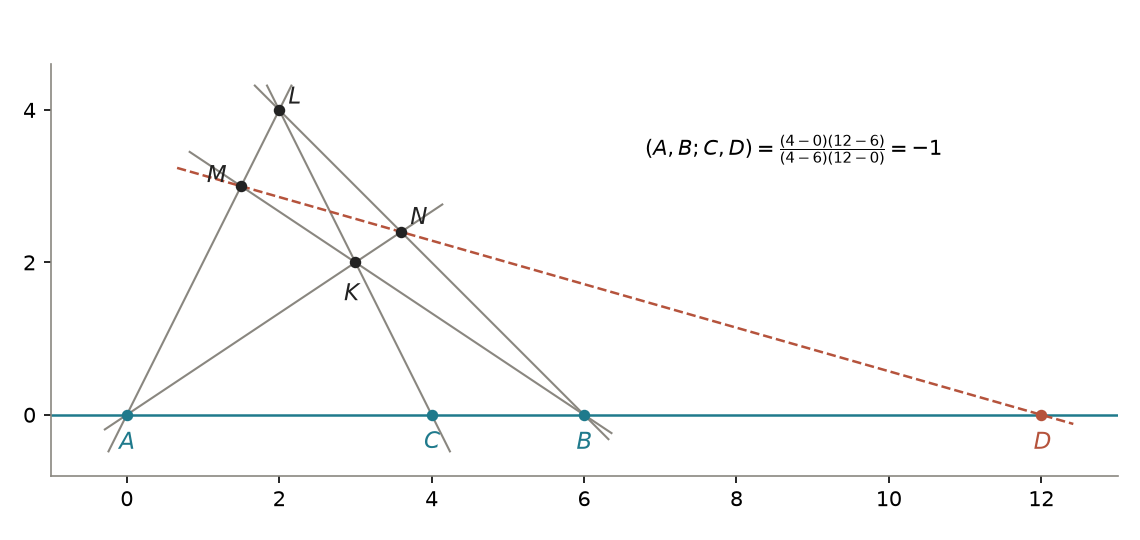
\includegraphics[width=.9\linewidth]{figuras/proyectivas/c1_conjugado_armonico.png}
\caption{Construcción del conjugado armónico con el cuadrilátero completo \(L,M,N,K\):
\(A=(0,0)\), \(B=(6,0)\), \(C=(4,0)\), \(L=(2,4)\), \(K=(3,2)\), \(M=BK\cap LA=(1{,}5;\ 3)\),
\(N=AK\cap LB=(3{,}6;\ 2{,}4)\) y \(D=MN\cap AB=(12,0)\). Generada con
\texttt{apunte/scripts/capc1\_conjugado\_armonico.py}.}
\label{fig:c1-conjugado-armonico}
\end{figure}

\begin{ejemplo}[Conjugado armónico con coordenadas]\label{ej:c1-conjugado-armonico}
Sean \(A=(0,0)\), \(B=(6,0)\) y \(C=(4,0)\) sobre el eje \(x\), con la abscisa como coordenada
afín. La fórmula da \(d=\dfrac{6\cdot4}{2\cdot4-6}=12\), y en efecto
\[
  (0,6;4,12)=\frac{(4-0)(12-6)}{(4-6)(12-0)}=\frac{24}{-24}=-1 .
\]
\(C\) está dentro de \(AB\), más cerca de \(B\), y \(D\) quedó afuera, del lado de \(B\). La
construcción de la figura~\ref{fig:c1-conjugado-armonico} da lo mismo con productos cruz
en homogéneas: con \(L=(2,4)\) y \(K=(3,2)\), el punto medio de \(LC\), resultan
\(M=(1{,}5;\ 3)\), \(N=(3{,}6;\ 2{,}4)\), y la recta \(MN\), de pendiente \(-2/7\), corta al eje en
\(x=1{,}5+3\cdot\tfrac72=12\). Por último, la homografía \(f(x)=\dfrac{2x+1}{x+3}\) del
ejemplo~\ref{ej:c1-razon-doble} lleva \(0,6,4,12\) a \(\tfrac13,\tfrac{13}9,\tfrac97,\tfrac53\), y
\[
  \Bigl(\tfrac13,\tfrac{13}9;\tfrac97,\tfrac53\Bigr)
  =\frac{\bigl(\tfrac97-\tfrac13\bigr)\bigl(\tfrac53-\tfrac{13}9\bigr)}
        {\bigl(\tfrac97-\tfrac{13}9\bigr)\bigl(\tfrac53-\tfrac13\bigr)}
  =\frac{\tfrac{20}{21}\cdot\tfrac29}{-\tfrac{10}{63}\cdot\tfrac43}
  =\frac{40/189}{-40/189}=-1 :
\]
la cuaterna sigue siendo armónica, aunque \(C\) ya no divide al segmento en la misma razón.
\end{ejemplo}

En una homología armónica (sección~\ref{sec:homografia-fijos}), cada punto y su imagen son
conjugados armónicos respecto del centro y del corte de su recta con el eje; es lo que
comprueba la razón doble \((D,D';O,X)=-1\) en el ejercicio del pentágono de la unidad
interactiva.

\begin{atencion}[Tres \enquote{conjugados} distintos]
El conjugado armónico no tiene relación con la conjugación de matrices
(sección~\ref{sec:conjugacion}) ni con el conjugado complejo
(sección~\ref{sec:conjugado-complejo}): es la misma palabra para tres ideas distintas. El
glosario de la sección~\ref{sec:glosario} las separa.
\end{atencion}

\subsection{Cuatro puntos determinan la homografía}\label{sec:cuatro-puntos}

¿Cuántos puntos de una pared hay que reconocer en su foto para poder deshacer la perspectiva?
Con tres alcanzaba para una afinidad (proposición~\ref{prop:06-tres-puntos}); la perspectiva pide
uno más.

\paragraph{Conteo.} Cada correspondencia \(p_i\mapsto p_i'\) aporta dos ecuaciones
(\(X/W=x_i'\), \(Y/W=y_i'\)). Cuatro correspondencias dan ocho ecuaciones para ocho
incógnitas. La condición es que ni entre los cuatro puntos de partida ni entre los cuatro de
llegada haya tres alineados (con el determinante se verifica).

\paragraph{Construcción.} En lugar de resolver el sistema \(8\times8\) se pasa por un
\emph{cuadrilátero patrón}:
\[
  e_1=\begin{pmatrix}1\\0\\0\end{pmatrix},\quad
  e_2=\begin{pmatrix}0\\1\\0\end{pmatrix},\quad
  e_3=\begin{pmatrix}0\\0\\1\end{pmatrix},\quad
  e_4=\begin{pmatrix}1\\1\\1\end{pmatrix}=e_1+e_2+e_3 .
\]
Dados cuatro puntos \(p_1,p_2,p_3,p_4\) sin tres alineados, se busca una matriz \(K\) con
\(Ke_i\sim p_i\) para \(i=1,\dots,4\):
\begin{enumerate}
  \item Se forma \(M=[\,p_1\ p_2\ p_3\,]\) con los tres primeros puntos como columnas. Como
  \(Me_i\) es la \(i\)-ésima columna, ya se cumple \(Me_i=p_i\) para \(i\le3\). Pero
  \(Me_4=p_1+p_2+p_3\), que en general no es \(p_4\).
  \item Como cada columna representa su punto \emph{a menos de escala}, se la puede
  multiplicar por un número sin cambiar a dónde va \(e_i\). Se eligen \(\mu_1,\mu_2,
  \mu_3\) tales que
  \[
    \mu_1p_1+\mu_2p_2+\mu_3p_3=p_4
    \qquad\Longleftrightarrow\qquad
    \mu=M^{-1}p_4 .
  \]
  \item La matriz buscada es \(K=[\,\mu_1p_1\ \ \mu_2p_2\ \ \mu_3p_3\,]\):
  las tres primeras columnas siguen representando \(p_1,p_2,p_3\) y su suma es \(p_4\).
\end{enumerate}

\begin{resultado}[Homografía que lleva un cuadrilátero sobre otro]
Sean \(K_1\) la matriz del patrón para los puntos de partida \(p_1,\dots,p_4\) y \(K_2\) la
del patrón para los puntos de llegada \(p_1',\dots,p_4'\). Entonces
\[
  \boxed{H=K_2K_1^{-1}}
\]
es la única homografía (a menos de escala) con \(Hp_i\sim p_i'\), \(i=1,\dots,4\).
Se lee de derecha a izquierda: \(K_1^{-1}\) lleva el cuadrilátero de partida al patrón, y
\(K_2\) lleva el patrón al cuadrilátero de llegada.
\end{resultado}

Es el mismo esquema de la afinidad determinada por tres puntos de control
(proposición~\ref{prop:06-tres-puntos}, \(A=P'P^{-1}\)), con un punto más para absorber la
perspectiva. Los \(\mu_i\), invisibles punto a punto, son precisamente los
grados de libertad que faltaban.

\subsection{Puntos fijos y rectas fijas de una homografía}\label{sec:homografia-fijos}

¿Hay algún punto que una homografía deje en su lugar? Saberlo dice qué tipo de
transformación es: un giro alrededor de un punto, un espejo, o una perspectiva más general.

Los puntos fijos de una homografía son autovectores; la teoría general de autovalores y
autovectores se desarrolla en las secciones~\ref{sec:autovalores} y~\ref{sec:autovalores-geom}.
Un punto \(p\) es fijo si
\(Hp\sim p\), es decir si existe \(\lambda\neq0\) con \(Hp=\lambda p\): \emph{los puntos
fijos son los autovectores reales de \(H\)}. Se calculan así: se buscan las raíces reales de
\(\det(H-\lambda I)=0\) y, para cada una, se toma el producto cruz de dos filas de
\(H-\lambda I\). Ese vector es perpendicular a las dos filas; cuando \(H-\lambda I\) tiene
rango \(2\), la tercera fila es combinación de las otras dos y el producto cruz anula a toda
la matriz, es decir, resuelve \((H-\lambda I)p=0\).

\begin{resultado}[Existencia de punto fijo]
Toda homografía del plano tiene al menos un punto fijo, porque el polinomio característico
es de grado \(3\). Es ordinario si el autovector tiene tercera coordenada no nula, e ideal
(una dirección fija) si la tercera coordenada es cero. Una raíz doble con producto cruz de
filas nulo significa toda una recta de puntos fijos.
\end{resultado}

\paragraph{Rectas fijas.} Como las rectas se transforman con \(H^{-T}\), una recta es fija
si es autovector de \(H^{T}\); se encuentra con el producto cruz de dos filas de
\(H^{T}-\lambda I\) (o sea, de dos columnas de \(H-\lambda I\)). Una recta fija de autovalor
\(\lambda'\) pasa por todos los puntos fijos de autovalor \(\lambda\neq\lambda'\).

\paragraph{Clasificación por autovalores.}
\begin{itemize}
  \item \textbf{Tres autovalores reales distintos:} tres puntos fijos no alineados y tres
  rectas fijas, los lados de ese triángulo.
  \item \textbf{Un real y dos complejos conjugados} (\(\lambda\) y \(\bar\lambda\), en el sentido de la sección~\ref{sec:conjugado-complejo})\textbf{:} un único punto fijo real y una única
  recta fija real que no pasa por él. En coordenadas adecuadas es una rotación alrededor del
  punto fijo, con la recta fija en el papel de recta ideal.
  \item \textbf{Un autovalor doble con producto cruz de filas nulo:} una recta entera de
  puntos fijos (el \emph{eje}) y un punto fijo aislado (el \emph{centro}) con el otro
  autovalor. Es una \emph{homología}. Si los dos autovalores son opuestos, \(H^2\sim I\): la
  homología es \emph{armónica}, una involución, como una reflexión.
\end{itemize}

\subsection{Aplicación: enderezar la foto de una fachada}\label{sec:c1-aplicacion-fachada}

Tenemos una foto de una pared, sacada de costado y un poco desde abajo, y queremos saber cuánto
mide una puerta de esa pared sin ir a medirla. De la pared conocemos una sola cosa: tiene una
ventana rectangular de \(1{,}50\ \mathrm{m}\) de ancho por \(1{,}20\ \mathrm{m}\) de alto, que
medimos con una cinta. En la foto la ventana no sale rectangular: es un cuadrilátero con los
lados opuestos inclinados distinto, y la puerta, que está más lejos de la cámara, sale más
chica de lo que es. ¿Podemos usar la ventana como patrón para enderezar la pared entera y medir
la puerta sobre la pared enderezada? Por la sección~\ref{sec:cuatro-puntos}, sí: los cuatro
vértices de la ventana, en la foto y en la pared, determinan la homografía que lleva una a la
otra.

\begin{idea}[Esto lo vas a usar en Topografía]
Enderezar la foto de una superficie plana a partir de puntos cuyas medidas se conocen se llama
\emph{rectificar} la foto. Sirve para dibujar fachadas y para medir sobre cualquier superficie
plana fotografiada sin recorrerla con la cinta.
\end{idea}

\paragraph{Dos sistemas de coordenadas.} En la foto usamos, como en la ortofoto del
capítulo~\ref{cap:afines} (sección~\ref{sec:aplicacion-ortofoto}), la columna \(c\) y la fila
\(f\) de cada píxel, con origen en el vértice superior izquierdo y \emph{la fila creciendo hacia
abajo}. En la pared usamos metros: \(x\) hacia la derecha e \(y\) hacia arriba, con origen en el
vértice inferior izquierdo de la ventana. Buscamos la matriz \(H\) de \(3\times3\) que lleva
\((c,f,1)^T\) a un múltiplo de \((x,y,1)^T\).

\paragraph{Datos.} Son sintéticos, generados por el script
\texttt{apunte/scripts/c1\_proyectivas.py}. El script parte de una pared de juguete (la ventana de
\(1{,}50\times1{,}20\ \mathrm{m}\) y una puerta de \(0{,}90\times2{,}05\ \mathrm{m}\)), la
fotografía con una homografía conocida, la que produciría una cámara de distancia focal
\(1300\) píxeles girada \(40^\circ\) respecto de la pared y levantada \(12^\circ\), y a cada
vértice le suma un error al azar de medio píxel (semilla \(2026\)), redondeando al décimo de
píxel, como cuando se marcan los vértices a mano sobre la pantalla. Las medidas de la puerta no
entran en el cálculo: las guardamos para comparar al final.
\begin{center}
\begin{tabular}{lcc}
\toprule
punto & foto \((c;\,f)\) (px) & pared \((x;\,y)\) (m)\\
\midrule
\(V_1\) ventana, abajo a la izquierda & \(93{,}3;\ 692{,}1\) & \(0;\ 0\)\\
\(V_2\) ventana, abajo a la derecha & \(567{,}7;\ 730{,}9\) & \(1{,}50;\ 0\)\\
\(V_3\) ventana, arriba a la derecha & \(581{,}0;\ 405{,}2\) & \(1{,}50;\ 1{,}20\)\\
\(V_4\) ventana, arriba a la izquierda & \(139{,}2;\ 290{,}2\) & \(0;\ 1{,}20\)\\
\midrule
\(P_1\) puerta, abajo a la izquierda & \(768{,}2;\ 997{,}9\) & a medir\\
\(P_2\) puerta, abajo a la derecha & \(935{,}5;\ 985{,}7\) & a medir\\
\(P_3\) puerta, arriba a la derecha & \(925{,}3;\ 516{,}3\) & a medir\\
\(P_4\) puerta, arriba a la izquierda & \(770{,}9;\ 477{,}9\) & a medir\\
\bottomrule
\end{tabular}
\end{center}

\begin{figure}[htbp]
\centering
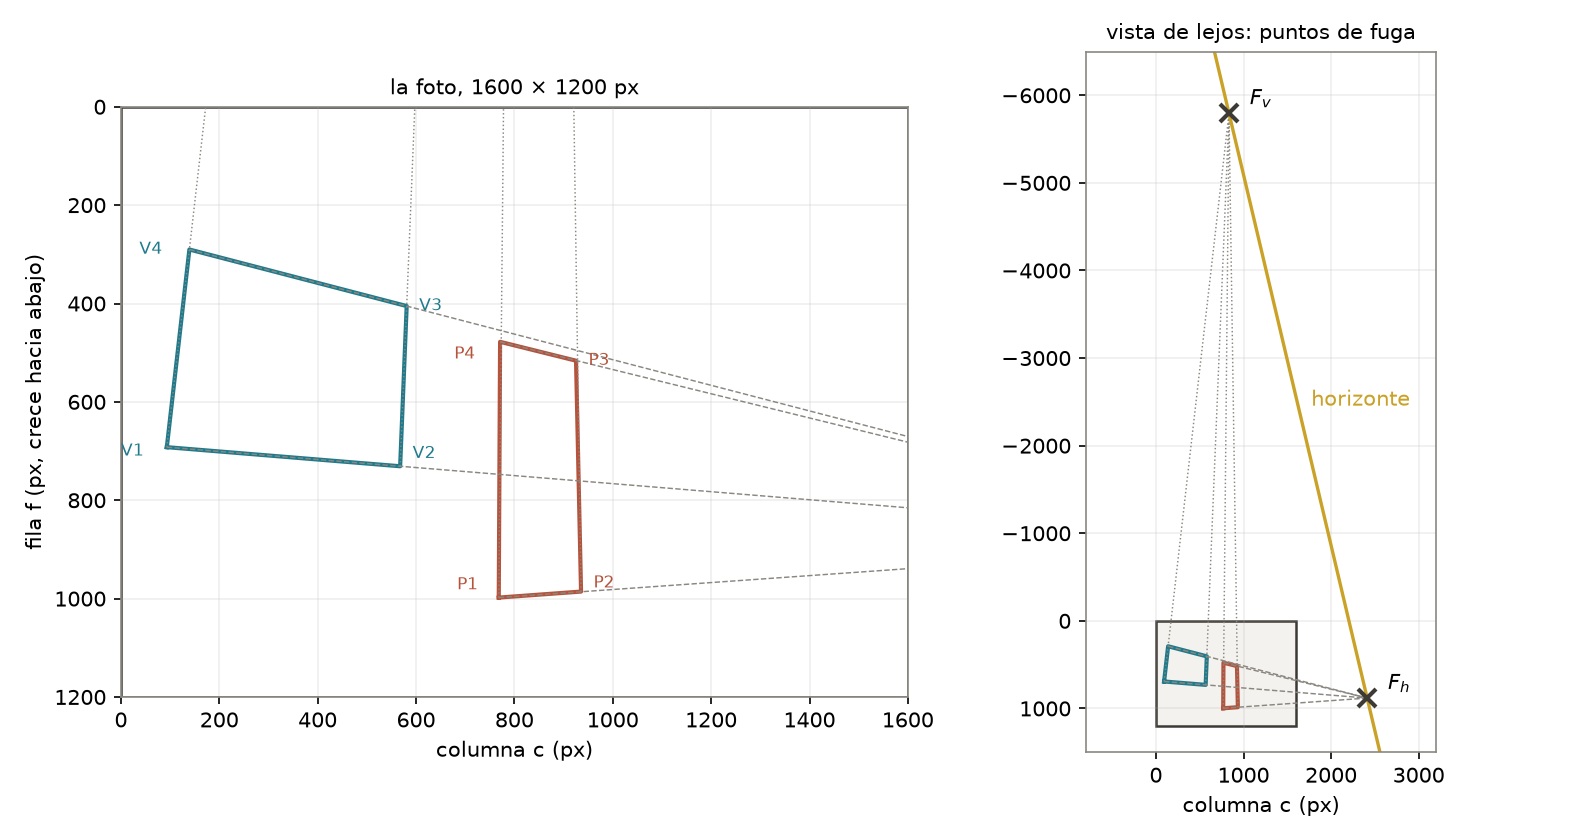
\includegraphics[width=\linewidth]{figuras/proyectivas/c1_fachada_foto.png}
\caption{Izquierda: la foto sintética de la fachada, con la ventana (\(V_1\) a \(V_4\)) y la
puerta (\(P_1\) a \(P_4\)); en gris, las prolongaciones de los lados. Derecha: la misma foto vista
de lejos. Los lados que en la pared son horizontales se cortan en el punto de fuga \(F_h\), los
verticales en \(F_v\), y la recta que los une es el horizonte, la recta que \(H\) manda al
infinito. Generada con \texttt{apunte/scripts/c1\_proyectivas.py}.}
\label{fig:c1-fachada-foto}
\end{figure}

\paragraph{Lo que la foto no respeta.} Medidos contra la horizontal de la foto, el lado de
abajo de la ventana baja \(4{,}68^\circ\) hacia la derecha y el de arriba \(14{,}59^\circ\): en
la pared son paralelos y en la foto no. Los lados verticales forman \(83{,}48^\circ\) y
\(87{,}66^\circ\) con la horizontal: tampoco son paralelos. ¿Dónde se cortan? Con las rectas en
coordenadas homogéneas, la recta por dos puntos y el punto común a dos rectas se calculan con
el producto cruz. Los lados de abajo y de arriba se cortan en el punto de fuga
\(F_h=(2411{,}6;\ 881{,}7)\), fuera de la foto a la derecha; los lados verticales, en
\(F_v=(834{,}2;\ -5795{,}1)\), muy por encima de la foto, porque la cámara mira hacia arriba
(figura~\ref{fig:c1-fachada-foto}). Si quisiéramos medir la puerta con una regla sobre la foto,
usando como escala la ventana (\(1{,}50\ \mathrm{m}\) en los \(476{,}0\) px del lado de abajo y
\(1{,}20\ \mathrm{m}\) en los \(404{,}5\) px del lado izquierdo), los \(167{,}7\) px del lado de
abajo de la puerta darían \(0{,}53\ \mathrm{m}\) y los \(520{,}0\) px del lado izquierdo,
\(1{,}54\ \mathrm{m}\): \(37\ \mathrm{cm}\) de menos en el ancho y \(51\ \mathrm{cm}\) en el
alto. En la foto la escala cambia de un punto a otro.

\paragraph{Ocho ecuaciones lineales.} Escribimos la homografía buscada coordenada por
coordenada, con \(h_{ij}\) la entrada de la fila \(i\) y la columna \(j\) de \(H\):
\[
  x=\frac{h_{11}c+h_{12}f+h_{13}}{h_{31}c+h_{32}f+h_{33}},
  \qquad
  y=\frac{h_{21}c+h_{22}f+h_{23}}{h_{31}c+h_{32}f+h_{33}} .
\]
Como \(H\) y \(\mu H\) dan la misma transformación, podemos elegir la escala: fijamos
\(h_{33}=1\). (Esa elección solo falla si \(h_{33}=0\), cuando el píxel \((0,0)\) va al infinito;
no es el caso de una foto en la que la pared ocupa el cuadro.) Pasando el denominador a la
izquierda y ordenando, cada vértice da dos ecuaciones \emph{lineales} en las ocho incógnitas:
\[
\begin{aligned}
  h_{11}c+h_{12}f+h_{13}-h_{31}\,c\,x-h_{32}\,f\,x&=x,\\
  h_{21}c+h_{22}f+h_{23}-h_{31}\,c\,y-h_{32}\,f\,y&=y .
\end{aligned}
\]
Es la \emph{transformación lineal directa} (en inglés, DLT): directa porque el problema, que
parecía de cocientes, quedó como un sistema lineal común. Por ejemplo, \(V_2\), con
\((c;\,f)=(567{,}7;\ 730{,}9)\) y \((x;\,y)=(1{,}5;\ 0)\), aporta las filas
\[
\begin{aligned}
  567{,}7\,h_{11}+730{,}9\,h_{12}+h_{13}-851{,}55\,h_{31}-1096{,}35\,h_{32}&=1{,}5,\\
  567{,}7\,h_{21}+730{,}9\,h_{22}+h_{23}&=0 .
\end{aligned}
\]
Con los cuatro vértices de la ventana queda un sistema de \(8\times8\), con solución única
porque no hay tres vértices alineados. Resulta
\[
  H=10^{-3}\begin{pmatrix}
  2{,}5710&0{,}2936&-443{,}09\\
  0{,}2342&-2{,}8633&1959{,}87\\
  -0{,}4539&0{,}1072&1000
  \end{pmatrix}.
\]
El script comprueba que el método del patrón de la sección~\ref{sec:cuatro-puntos},
\(H=K_2K_1^{-1}\) normalizada con \(h_{33}=1\), da la misma matriz, y que \(H\) lleva los cuatro
vértices de la ventana a \((0;\ 0)\), \((1{,}5;\ 0)\), \((1{,}5;\ 1{,}2)\) y \((0;\ 1{,}2)\).

\paragraph{El horizonte.} La tercera fila de \(H\) es la recta de la foto que se va al infinito
(sección~\ref{sec:jerarquia}): \(-0{,}4539\,c+0{,}1072\,f+1000=0\). Tiene que pasar por \(F_h\) y
por \(F_v\), porque las imágenes de los lados de la ventana son paralelas y sus puntos comunes
están en el infinito. El script calcula la recta \(F_h\times F_v\) y comprueba que es la misma.
Es el horizonte dorado de la figura~\ref{fig:c1-fachada-foto}.

\paragraph{Las rectas siguen rectas, las razones simples no.} Tomemos en la foto el punto medio
del borde izquierdo de la puerta, \((769{,}55;\ 737{,}9)\), a mitad de camino entre \(P_1\) y
\(P_4\). \(H\) lo lleva a \((2{,}401;\ 0{,}037)\), y el determinante de las ternas de las tres
imágenes (los extremos y ese punto) da cero: siguen alineadas. Pero el punto ya no está a mitad
de altura: queda a \(0{,}480\) del recorrido, contando desde abajo. Lo que la foto muestra como
mitad, en la pared no lo es.

\paragraph{La razón doble se conserva.} Prolonguemos en la foto el lado de abajo de la ventana,
la recta del alféizar (el borde inferior de la ventana). Corta a los bordes verticales de la
puerta en dos puntos, \(Q\) y \(R\), que se calculan otra vez con productos cruz. Sobre esa recta
de la foto, la columna \(c\) sirve de coordenada afín, y los cuatro puntos \(V_1,V_2,Q,R\) tienen
\(c=93{,}3;\ 567{,}7;\ 769{,}5;\ 930{,}6\). En la pared enderezada caen sobre la recta \(y=0\), en
\(x=0;\ 1{,}5;\ 2{,}401;\ 3{,}296\). La razón doble
(definición~\ref{def:c1-razon-doble}) vale
\[
  (V_1,V_2;Q,R)=1{,}4523
\]
en las dos, con todas las cifras que calcula el script, como asegura la
proposición~\ref{prop:c1-razon-doble}. La razón simple, en cambio, cambia: \(V_1V_2/V_1Q\) es
\(0{,}702\) en la foto y \(0{,}625\) en la pared. En la pared verdadera, con los bordes de la
puerta en \(x=2{,}4\) y \(x=3{,}3\), la razón doble es \(16/11\approx1{,}4545\); la diferencia con
\(1{,}4523\) es el error de medio píxel de los vértices marcados.

\begin{figure}[htbp]
\centering
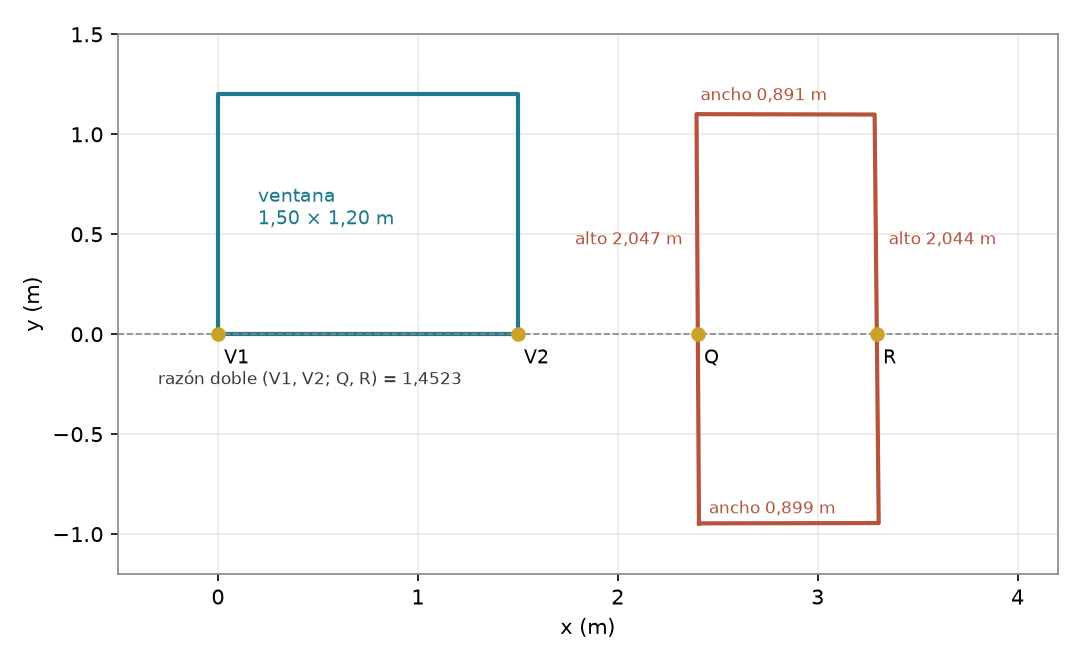
\includegraphics[width=.92\linewidth]{figuras/proyectivas/c1_fachada_enderezada.png}
\caption{La pared enderezada por \(H\): la ventana vuelve a ser el rectángulo de
\(1{,}50\times1{,}20\ \mathrm{m}\) y la puerta aparece con sus medidas. Los puntos dorados son
\(V_1\), \(V_2\), \(Q\) y \(R\) sobre la recta \(y=0\), la del alféizar, con la misma razón doble
que en la foto. Generada con \texttt{apunte/scripts/c1\_proyectivas.py}.}
\label{fig:c1-fachada-enderezada}
\end{figure}

\paragraph{La puerta, medida.} Aplicando \(H\) a \(P_1,\dots,P_4\) obtenemos, en metros,
\[
  P_1\mapsto(2{,}406;\ -0{,}946),\quad P_2\mapsto(3{,}306;\ -0{,}945),\quad
  P_3\mapsto(3{,}285;\ 1{,}099),\quad P_4\mapsto(2{,}394;\ 1{,}101).
\]
Los lados de abajo y de arriba miden \(0{,}899\) y \(0{,}891\ \mathrm{m}\), y los bordes
izquierdo y derecho \(2{,}047\) y \(2{,}044\ \mathrm{m}\)
(figura~\ref{fig:c1-fachada-enderezada}). Promediando, la puerta mide \(0{,}895\ \mathrm{m}\) de
ancho por \(2{,}045\ \mathrm{m}\) de alto. Las medidas con que el script armó la pared son
\(0{,}90\) y \(2{,}05\ \mathrm{m}\): la diferencia, de unos \(5\ \mathrm{mm}\), viene del medio
píxel de error al marcar los ocho vértices. Los bordes verticales de la puerta, que en la foto
forman entre sí \(1{,}54^\circ\), en la pared enderezada forman \(0{,}23^\circ\): casi
paralelos, y lo que falta también es error de marcado.

\begin{atencion}[Una pared, no un edificio]
La homografía endereza \emph{un plano}. Todo lo que está sobre la pared (ventanas, puertas,
juntas de ladrillos) queda bien medido; lo que sobresale de ella (un balcón, el marco de la
ventana si está hundido) no, porque no está en el plano que fijaron los cuatro vértices.
\end{atencion}

\unidadInteractiva{05_proyectivas}{Proyectivas: la perspectiva de una cámara y el pentágono regular}{Explorá: en «caso precargado» elegí «foto de dron: cámara inclinada (k)» y mové el deslizador «k (inclinación, h\(_{32}\))». Con \(k=0\) la tercera fila de la matriz es \((0\ \ 0\ \ 1)\): la transformación es afín y las rectas \(x=\) constante siguen paralelas. Con cualquier otro \(k\) convergen al punto de fuga marcado con una cruz, como los bordes verticales de la puerta en la foto de la fachada.}

\section{En profundidad}

Resolvemos caso por caso el ejercicio del pentágono regular.

\subsection{El ejercicio del pentágono regular}

\begin{enunciado}[El quinto vértice de un pentágono regular]
Tomar un pentágono \emph{regular} \(ABCDE\). Una transformación proyectiva queda definida
por cuatro puntos, así que se prescriben cuatro vértices y sus imágenes (otros cuatro
vértices) y se pregunta \emph{a dónde cae el quinto}. Hay tres casos, y sus combinaciones
con las rotaciones del pentágono:
\begin{enumerate}[label=(\alph*)]
  \item no intercambiar ningún vértice: solo \enquote{correr} el pentágono;
  \item intercambiar dos vértices adyacentes;
  \item intercambiar dos vértices no adyacentes.
\end{enumerate}
Para cada transformación, determinar si tiene punto fijo (un autovector de la matriz).
\end{enunciado}

Se toma el pentágono regular inscripto en la circunferencia unidad,
centrado en el origen y con un vértice arriba. Conviene centrarlo en el origen:
en el caso más simple el punto fijo es el centro, cuyo autovector es \((0,0,1)^T\).
\begin{gather*}
  A=(0,\,1),\qquad B=(-0{,}9511;\ 0{,}3090),\qquad C=(-0{,}5878;\ -0{,}8090),\\
  D=(0{,}5878;\ -0{,}8090),\qquad E=(0{,}9511;\ 0{,}3090).
\end{gather*}
Las coordenadas son irracionales (\(\cos72^\circ=\frac{\sqrt5-1}{4}\)), así que las
matrices se calculan con cuatro decimales y se verifican en NumPy (apéndice~\ref{ap:pentagono}).
En los tres casos se usa \(H=K_2K_1^{-1}\) con \(K_1\) el patrón de \(ABCD\), y se
normaliza \(h_{33}=1\).

\begin{center}
\begin{tikzpicture}[scale=1.9]
  \draw[linegray!40,very thin] (-1.6,-1.4) grid[step=.5] (1.6,1.3);
  \draw[axisline,-{Latex[length=2.2mm]}] (-1.7,0)--(1.7,0) node[right] {$x$};
  \draw[axisline,-{Latex[length=2.2mm]}] (0,-1.45)--(0,1.35) node[above] {$y$};
  \draw[linegray,densely dotted] (0,0) circle (1);
  \draw[teal,line width=1.05pt,fill=teallight!45] (0,1)--(-0.9511,0.3090)--(-0.5878,-0.8090)--(0.5878,-0.8090)--(0.9511,0.3090)--cycle;
  \foreach \p/\n/\pos in {(0,1)/A/above,(-0.9511,0.3090)/B/left,(-0.5878,-0.8090)/C/{below left},(0.5878,-0.8090)/D/{below right},(0.9511,0.3090)/E/right}
    \fill[teal] \p circle (1.2pt) node[\pos,font=\small,text=tealdark] {$\n$};
  \fill[ink] (0,0) circle (1.2pt) node[below right,font=\scriptsize] {$O$};
  % caso (c): imagen C B A D E'
  \draw[rust,line width=1pt] (-0.5878,-0.8090)--(-0.9511,0.3090)--(0,1)--(0.5878,-0.8090)--(0,-1.2361)--cycle;
  \fill[rust] (0,-1.2361) circle (1.4pt) node[right=2pt,font=\small,text=rust,labelback] {$E'_c=(0;\ -1{,}2361)$};
  % eje BD
  \draw[dashed,tealdark,line width=.8pt] ($(-0.9511,0.3090)!-0.35!(0.5878,-0.8090)$)--($(-0.9511,0.3090)!1.35!(0.5878,-0.8090)$) node[right,font=\scriptsize,text=tealdark] {eje $BD$};
  % recta AC (contiene al centro)
  \draw[dotted,gold!70!black,line width=.8pt] ($(0,1)!-0.3!(-0.5878,-0.8090)$)--($(0,1)!1.3!(-0.5878,-0.8090)$);
  \node[gold!60!black,font=\scriptsize,labelback,anchor=east] at (-0.55,-1.3) {hacia $O_c=(-1{,}54;\ -3{,}74)$};
\end{tikzpicture}
\end{center}

\paragraph{(a) Sin intercambio: \(A\mapsto B,\ B\mapsto C,\ C\mapsto D,\ D\mapsto E\).}
Los cuatro pares son compatibles con la rotación de \(72^\circ\) alrededor de \(O\), que es
una isometría y por lo tanto una homografía. Como la homografía es única, \emph{es} esa
rotación:
\[
  H_a=\begin{pmatrix}0{,}3090&-0{,}9511&0\\0{,}9511&0{,}3090&0\\0&0&1\end{pmatrix},
  \qquad H_aE=A .
\]
El quinto vértice cae en \(A\): el pentágono regular sí \enquote{cierra}. Autovalores \(1\) y
\(e^{\pm i\,72^\circ}\); único punto fijo real \(O=(0,0)\), obtenido como producto cruz de
las dos primeras filas de \(H_a-I\):
\[
  (-0{,}691;\ -0{,}951;\ 0)\times(0{,}951;\ -0{,}691;\ 0)=(0;\ 0;\ 1{,}382)\sim(0,0,1)^T .
\]
La recta ideal es fija (es afín) y ninguna otra.

\paragraph{(b) Intercambio de adyacentes: \(A\leftrightarrow B\), \(C\) y \(D\) quietos.}
\[
  H_b=\begin{pmatrix}-5{,}8541&-4{,}9798&-4{,}0287\\0&-1&3{,}9271\\0&8{,}4721&1\end{pmatrix},
  \qquad E\mapsto E'_b=(-3{,}0777;\ 1{,}0000).
\]
Autovalores \(5{,}8541\) (simple) y \(-5{,}8541\) (doble). Para el doble, el producto cruz de
cualquier par de filas de \(H_b+5{,}8541I\) es nulo: hay toda una recta de puntos fijos, que es
la recta \(CD\) (\(y=-0{,}8090\)), lógico porque \(C\) y \(D\) quedan quietos. El autovalor
simple da el centro, \(O_b=(-0{,}5878;\ 0{,}5729)\), que está sobre la recta \(AB\) (la recta
\(AB\) va a sí misma porque sus extremos se intercambian). Como los autovalores son
opuestos, \(H_b^2\sim I\): es una \emph{homología armónica}, un \enquote{espejo proyectivo} de eje
\(CD\) y centro \(O_b\). La recta que se va al infinito es \(y=-0{,}1180\), que
\emph{atraviesa} el pentágono (\(W\) vale \(9{,}47;\ 3{,}62;\ -5{,}85;\ -5{,}85;\ 3{,}62\) en
\(A,\dots,E\)): los lados \(BC\) y \(DE\) la cruzan y la imagen del pentágono se parte en
dos semirrectas por lado.

\paragraph{(c) Intercambio de no adyacentes: \(A\leftrightarrow C\), \(B\) y \(D\) quietos.}
\[
  H_c=\begin{pmatrix}0{,}4271&-0{,}5878&-0{,}2245\\-1{,}0368&-0{,}5729&-0{,}5451\\0{,}2775&0{,}3820&1\end{pmatrix},
  \qquad E\mapsto E'_c=(0;\ -1{,}2361).
\]
Autovalores \(0{,}8541\) (doble) y \(-0{,}8541\). Eje de puntos fijos: la recta \(BD\)
(\(0{,}7265x+y+0{,}3820=0\)); centro \(O_c=(-1{,}5388;\ -3{,}7361)\), sobre la prolongación de
\(AC\), obtenido como producto cruz de las dos primeras filas de \(H_c+0{,}8541I\):
\((1{,}2812;\ -0{,}5878;\ -0{,}2245)\times(-1{,}0368;\ 0{,}2812;\ -0{,}5451)=(0{,}3835;\ 0{,}9311;\ -0{,}2492)\sim
(-1{,}5388;\ -3{,}7361;\ 1)\). Otra vez \(H_c^2\sim I\): homología armónica de eje \(BD\). El
quinto vértice cae en \(E'_c=(0;\ -1{,}2361)\), sobre el eje de simetría, y como la recta que se
va al infinito (\(0{,}2775x+0{,}3820y+1=0\)) no toca el pentágono (\(W>0\) en los cinco
vértices), la imagen es el pentágono \(CBADE'_c\) de la figura, no convexo pero entero.

\paragraph{Combinaciones con rotaciones.} Cualquier otra correspondencia de cuatro vértices
sobre cuatro vértices es una de las tres anteriores seguida de una rotación \(H_a^k\), o una
reflexión del pentágono. Por ejemplo \(A\mapsto E,\ B\mapsto D,\ C\mapsto C,\ D\mapsto B\)
es la reflexión respecto del eje \(OC\) (afín, \(E\mapsto A\), todo el eje fijo y la
dirección perpendicular como punto fijo ideal). Componer (b) con la rotación da un único punto
fijo real y dos autovalores complejos; componer (c) con la rotación da tres autovalores
reales distintos y un triángulo invariante. El script de la sección~\ref{ap:pentagono}
permite verificarlo.

\begin{resultado}[Respuestas a la consigna]
\begin{itemize}
  \item Con \(A,B,C,D\) fijos como puntos de partida, sus imágenes son cuatro vértices
  distintos elegidos en orden entre cinco: hay \(5\cdot4\cdot3\cdot2=120\) correspondencias,
  todas bien definidas (el pentágono es convexo, nunca hay tres vértices alineados). Componer
  con las \(10\) simetrías del pentágono (\(5\) rotaciones y \(5\) reflexiones) agrupa esas
  \(120\) correspondencias en \(120/10=12\) familias. Dentro de una familia las homografías
  difieren en una simetría, así que basta estudiar un representante por familia: (a) está en
  la familia de la identidad, y (b) y (c) son representantes de otras dos.
  \item (a) es la rotación; el quinto vértice cae en un vértice y el punto fijo es el centro.
  \item (b) y (c) son homologías armónicas: una recta entera de puntos fijos, la que une los
  dos vértices que quedan quietos (el lado \(CD\) en (b), la diagonal \(BD\) en (c)), más un
  centro; el quinto vértice cae fuera del pentágono, en
  \((-3{,}08;\ 1)\) y \((0;\ -1{,}24)\) respectivamente. En (b) la imagen se parte; en (c) no.
  \item Siempre hay punto fijo: es el autovector real de \(H\), y se calcula con el producto
  cruz de dos filas de \(H-\lambda I\).
\end{itemize}
\end{resultado}

% Apéndice: pentágono regular: cuentas y script
\subsection{El pentágono}\label{cap:pentagono}\label{ap:pentagono}

Ternas homogéneas (cuatro decimales):
\[
A=\begin{pmatrix}0\\1\\1\end{pmatrix},\
B=\begin{pmatrix}-0{,}9511\\0{,}3090\\1\end{pmatrix},\
C=\begin{pmatrix}-0{,}5878\\-0{,}8090\\1\end{pmatrix},\
D=\begin{pmatrix}0{,}5878\\-0{,}8090\\1\end{pmatrix},\
E=\begin{pmatrix}0{,}9511\\0{,}3090\\1\end{pmatrix}.
\]

\subsubsection{Verificación de los tres casos}
\begin{center}\small
\begin{tabularx}{\textwidth}{>{\bfseries}l X X X}
\toprule
& (a) \(ABCD\to BCDE\) & (b) \(ABCD\to BACD\) & (c) \(ABCD\to CBAD\)\\
\midrule
\(HA\) & \(B\), \(W=1\) & \(B\), \(W=9{,}4721\) & \(C\), \(W=1{,}3820\)\\
\(HB\) & \(C\), \(W=1\) & \(A\), \(W=3{,}6180\) & \(B\), \(W=0{,}8541\)\\
\(HC\) & \(D\), \(W=1\) & \(C\), \(W=-5{,}8541\) & \(A\), \(W=0{,}5279\)\\
\(HD\) & \(E\), \(W=1\) & \(D\), \(W=-5{,}8541\) & \(D\), \(W=0{,}8541\)\\
\(HE\) & \(A\), \(W=1\) & \((-3{,}0777;\ 1)\), \(W=3{,}6180\) & \((0;\ -1{,}2361)\), \(W=1{,}3820\)\\
recta al infinito & ideal & \(y=-0{,}1180\) & \(0{,}2775x+0{,}3820y+1=0\)\\
autovalores & \(1,\ e^{\pm i72^\circ}\) & \(5{,}8541;\ -5{,}8541\ (\times2)\) &
\(-0{,}8541;\ 0{,}8541\ (\times2)\)\\
puntos fijos & \(O=(0,0)\) & eje \(CD\); centro \((-0{,}5878;\ 0{,}5729)\) &
eje \(BD\); centro \((-1{,}5388;\ -3{,}7361)\)\\
tipo & rotación (afín) & homología armónica, imagen partida & homología armónica\\
\bottomrule
\end{tabularx}
\end{center}

\subsubsection{Autovector por producto cruz, caso (c)}
Polinomio característico de \(H_c\): \(\lambda^3-0{,}8541\lambda^2-0{,}7295\lambda+0{,}6231\),
raíces \(0{,}8541\) (doble) y \(-0{,}8541\). Para \(\lambda=-0{,}8541\),
\[
H_c+0{,}8541\,I=\begin{pmatrix}1{,}2812&-0{,}5878&-0{,}2245\\-1{,}0368&0{,}2812&-0{,}5451\\0{,}2775&0{,}3820&1{,}8541\end{pmatrix},
\]
\[
\text{fila}_1\times\text{fila}_2=
\begin{pmatrix}(-0{,}5878)(-0{,}5451)-(-0{,}2245)(0{,}2812)\\(-0{,}2245)(-1{,}0368)-(1{,}2812)(-0{,}5451)\\(1{,}2812)(0{,}2812)-(-0{,}5878)(-1{,}0368)\end{pmatrix}
=\begin{pmatrix}0{,}3835\\0{,}9311\\-0{,}2492\end{pmatrix}\sim\begin{pmatrix}-1{,}5388\\-3{,}7361\\1\end{pmatrix}.
\]
Comprobación:
\[
  H_c\begin{pmatrix}-1{,}5388\\-3{,}7361\\1\end{pmatrix}=\begin{pmatrix}1{,}3143\\3{,}1909\\-0{,}8541\end{pmatrix}
  =-0{,}8541\begin{pmatrix}-1{,}5388\\-3{,}7361\\1\end{pmatrix}.
\]
Para \(\lambda=0{,}8541\) el producto cruz de cualquier par de filas de \(H_c-0{,}8541I\) da
\((0,0,0)\): raíz doble, toda la recta \(BD\) es de puntos fijos.

\subsubsection{Imagen partida, caso (b)}
\begin{center}
\begin{tikzpicture}[scale=1.15]
  \clip (-3.6,-2.2) rectangle (2.4,2.1);
  \draw[linegray!40,very thin] (-3.5,-2) grid[step=.5] (2,2);
  \draw[axisline,-{Latex[length=2.2mm]}] (-3.5,0)--(2.2,0) node[right] {$x$};
  \draw[axisline,-{Latex[length=2.2mm]}] (0,-2.1)--(0,2) node[above] {$y$};
  \draw[teal,line width=1pt,fill=teallight!45] (0,1)--(-0.9511,0.3090)--(-0.5878,-0.8090)--(0.5878,-0.8090)--(0.9511,0.3090)--cycle;
  \foreach \p/\n/\pos in {(0,1)/A/{above right},(-0.9511,0.3090)/B/{above left},(-0.5878,-0.8090)/C/{below left},(0.5878,-0.8090)/D/{below right},(0.9511,0.3090)/E/right}
    \fill[teal] \p circle (1.2pt) node[\pos,font=\small,text=tealdark] {$\n$};
  \draw[gold!80!black,dotted,line width=.9pt] (-3.6,-0.118)--(2.4,-0.118) node[pos=.08,above,font=\scriptsize,text=gold!60!black] {$y=-0{,}118$ (se va al infinito)};
  % imagen: segmentos AB, CD, E'B
  \draw[rust,line width=1pt] (0,1)--(-0.9511,0.3090);
  \draw[rust,line width=1pt] (-0.5878,-0.8090)--(0.5878,-0.8090);
  \draw[rust,line width=1pt] (-3.0777,1)--(-0.9511,0.3090);
  % imagen de BC: recta AC exterior al segmento AC
  \draw[rust,line width=1pt,-{Latex[length=1.8mm]}] (0,1)--(0.35,2.077);
  \draw[rust,line width=1pt,-{Latex[length=1.8mm]}] (-0.5878,-0.8090)--(-1.0,-2.077);
  % imagen de DE: recta D E' exterior al segmento
  \draw[rust,line width=1pt,-{Latex[length=1.8mm]}] (0.5878,-0.8090)--(2.4,-1.703);
  \draw[rust,line width=1pt,-{Latex[length=1.8mm]}] (-3.0777,1)--(-3.6,1.258);
  \fill[rust] (-3.0777,1) circle (1.4pt) node[above,font=\small,text=rust,labelback] {$E'_b=(-3{,}08;\ 1)$};
  \draw[dashed,tealdark,line width=.8pt] (-3.6,-0.809)--(2.4,-0.809) node[pos=.12,below,font=\scriptsize,text=tealdark] {eje $CD$ (puntos fijos)};
  \fill[ink] (-0.5878,0.5729) circle (1.4pt) node[left,font=\scriptsize,labelback] {$O_b$};
\end{tikzpicture}
\end{center}
Los lados \(AB\), \(CD\) y \(EA\) van a los segmentos \(BA\), \(CD\) y \(E'_bB\). Los lados
\(BC\) y \(DE\) cruzan la recta \(y=-0{,}118\) y sus imágenes son las semirrectas exteriores de
las rectas \(AC\) y \(DE'_b\).

\subsubsection{Script}
Reproduce todo lo anterior: patrón, homografía, imágenes, autovalores, autovector por
producto cruz de filas y verificación.
\begin{verbatim}
import numpy as np
np.set_printoptions(precision=4, suppress=True)
ang = np.deg2rad(90 + 72*np.arange(5))
V = np.c_[np.cos(ang), np.sin(ang), np.ones(5)]      # A..E como filas
A, B, C, D, E = V

def patron(P):                       # P: 4 ternas como columnas
    M = P[:, :3]; lam = np.linalg.solve(M, P[:, 3]); return M * lam
def homografia(src, dst):
    K1 = patron(np.column_stack(src)); K2 = patron(np.column_stack(dst))
    H = K2 @ np.linalg.inv(K1)
    return H / H[2, 2]

casos = {"a": (B, C, D, E), "b": (B, A, C, D), "c": (C, B, A, D)}
for k, dst in casos.items():
    H = homografia((A, B, C, D), dst); print("caso", k); print(H)
    w = H @ E; print(" E ->", w[:2] / w[2], " W =", round(w[2], 4))
    lams = np.linalg.eigvals(H); print(" autovalores", lams)
    for lam in lams[np.isreal(lams)].real:
        M = H - lam * np.eye(3)
        v = np.cross(M[0], M[1])        # producto cruz de dos filas
        if np.linalg.norm(v) < 1e-9:
            v = np.cross(M[0], M[2])
        if np.linalg.norm(v) < 1e-9:
            print(f"  lambda={lam:.4f}: raiz doble, recta fija")
            continue
        if abs(v[2]) > 1e-9:
            v = v / v[2]                # punto propio (x, y, 1)
        print(f"  lambda={lam:.4f}: punto fijo", v)
\end{verbatim}

\section{Ejercicios con solución}

Los ejercicios 1 a 5 usan el pentágono regular de la sección~\ref{ap:pentagono}; los dos
últimos, la foto de la fachada de la sección~\ref{sec:c1-aplicacion-fachada}.

\begin{ejercicio}
Verificá con el determinante que \(A,B,C\) del pentágono regular no están alineados y que
\(A,O,C\) tampoco (\(O\) el centro).
\solucion{\(\det[A\ B\ C]=1{,}3143\neq0\); \(\det[A\ O\ C]=-0{,}5878\neq0\).}
\end{ejercicio}

\begin{ejercicio}
Calculá la recta \(BD\) como producto vectorial de las ternas de \(B\) y \(D\). Comprobá que el
centro \(O_c=(-1{,}5388;\ -3{,}7361)\) \emph{no} está en ella.
\solucion{\(B\times D=(0{,}3090+0{,}8090;\ 0{,}5878+0{,}9511;\ 0{,}7694-0{,}1816)\cdot\) (a menos de
escala) \(\sim(0{,}7265;\ 1;\ 0{,}3820)\); en \(O_c\): \(-1{,}118-3{,}736+0{,}382=-4{,}47\neq0\).}
\end{ejercicio}

\begin{ejercicio}
Con \(H_c\), calculá la imagen del centro \(O\) y comprobá que no es \(O\): en el caso (c) el
centro del pentágono no queda fijo.
\solucion{\(H_c(0,0,1)^T=(-0{,}2245;\ -0{,}5451;\ 1)^T\): \(O\mapsto(-0{,}22;\ -0{,}55)\).}
\end{ejercicio}

\begin{ejercicio}
Calculá \(H_c^2\) y normalizá: tiene que dar la identidad. Interpretá el resultado.
\solucion{\(H_c^2=0{,}7295\,I\): a menos de escala, la identidad; \(H_c\) es una involución,
aplicarla dos veces es no hacer nada, como con una reflexión.}
\end{ejercicio}

\begin{ejercicio}
Construí la matriz \(K\) del patrón para el cuadrado \((0,0),(1,0),(1,1),(0,1)\), en ese orden.
¿Es afín la homografía que lleva el patrón al cuadrado? Explicá por qué.
\solucion{\(M=\begin{pmatrix}0&1&1\\0&0&1\\1&1&1\end{pmatrix}\), \(\lambda=(1,-1,1)\),
\(K=\begin{pmatrix}0&-1&1\\0&0&1\\1&-1&1\end{pmatrix}\). No es afín (última fila
\((1,-1,1)\)): el patrón contiene los puntos ideales \(e_1,e_2\) y los manda a puntos
propios, cosa que una afinidad nunca hace.}
\end{ejercicio}

\begin{ejercicio}
En la foto de la fachada, \(V_1\) y \(V_2\) tienen columnas \(c=93{,}3\) y \(c=567{,}7\), y el
punto de fuga de los lados horizontales, \(F_h\), tiene \(c=2411{,}6\). ¿En qué columna de la
foto está el punto medio del alféizar, el punto de la pared \((0{,}75;\ 0)\)? Usá que el punto
medio de un segmento y el punto impropio de su recta son conjugados armónicos respecto de los
extremos, y que la homografía conserva la razón doble. Compará con el promedio de las columnas
de \(V_1\) y \(V_2\).
\solucion{En la pared, \((V_1,V_2;\text{medio},\infty)=-1\); en la foto el punto impropio va a
\(F_h\), así que el punto buscado es el conjugado armónico de \(F_h\) respecto de \(V_1\) y
\(V_2\). Con origen en \(V_1\): \(b=567{,}7-93{,}3=474{,}4\), \(d=2411{,}6-93{,}3=2318{,}3\), y de
\((c-0)(d-b)=-(c-b)(d-0)\) sale \(c=\dfrac{bd}{2d-b}=\dfrac{474{,}4\cdot2318{,}3}{4162{,}2}=264{,}2\).
La columna es \(93{,}3+264{,}2=357{,}5\), la misma que da \(H^{-1}\) aplicada a \((0{,}75;\ 0)\).
El promedio de las columnas es \(330{,}5\): el punto medio de la pared está \(27\) píxeles más
lejos, del lado que se aleja de la cámara.}
\end{ejercicio}

\begin{ejercicio}
Calculá la razón doble \((0;\ 1{,}5;\ 2{,}4;\ 3{,}3)\) de los puntos \(V_1,V_2,Q,R\) de la pared
verdadera. ¿Por qué la foto da \(1{,}4523\)? ¿Qué daría la foto si los vértices se hubieran
marcado sin error?
\solucion{\(\dfrac{(2{,}4-0)(3{,}3-1{,}5)}{(2{,}4-1{,}5)(3{,}3-0)}=\dfrac{4{,}32}{2{,}97}=\dfrac{16}{11}\approx1{,}4545\).
La foto da \(1{,}4523\) porque sus vértices tienen medio píxel de error; \(H\) conserva la razón
doble de la foto, y por eso la pared enderezada da también \(1{,}4523\). Sin error, foto, pared
enderezada y pared verdadera darían las tres \(16/11\).}
\end{ejercicio}
